\documentclass{ximera}

%\usepackage{todonotes}

\newcommand{\todo}{}

\usepackage{esint} % for \oiint
\ifxake%%https://math.meta.stackexchange.com/questions/9973/how-do-you-render-a-closed-surface-double-integral
\renewcommand{\oiint}{{\large\bigcirc}\kern-1.56em\iint}
\fi


\graphicspath{
  {./}
  {ximeraTutorial/}
  {basicPhilosophy/}
  {functionsOfSeveralVariables/}
  {normalVectors/}
  {lagrangeMultipliers/}
  {vectorFields/}
  {greensTheorem/}
  {shapeOfThingsToCome/}
  {dotProducts/}
  {partialDerivativesAndTheGradientVector/}
  {../productAndQuotientRules/exercises/}
  {../normalVectors/exercisesParametricPlots/}
  {../continuityOfFunctionsOfSeveralVariables/exercises/}
  {../partialDerivativesAndTheGradientVector/exercises/}
  {../directionalDerivativeAndChainRule/exercises/}
  {../commonCoordinates/exercisesCylindricalCoordinates/}
  {../commonCoordinates/exercisesSphericalCoordinates/}
  {../greensTheorem/exercisesCurlAndLineIntegrals/}
  {../greensTheorem/exercisesDivergenceAndLineIntegrals/}
  {../shapeOfThingsToCome/exercisesDivergenceTheorem/}
  {../greensTheorem/}
  {../shapeOfThingsToCome/}
  {../separableDifferentialEquations/exercises/}
  {vectorFields/}
}

\newcommand{\mooculus}{\textsf{\textbf{MOOC}\textnormal{\textsf{ULUS}}}}

\usepackage{tkz-euclide}
\usepackage{tikz}
\usepackage{tikz-cd}
\usetikzlibrary{arrows}
\tikzset{>=stealth,commutative diagrams/.cd,
  arrow style=tikz,diagrams={>=stealth}} %% cool arrow head
\tikzset{shorten <>/.style={ shorten >=#1, shorten <=#1 } } %% allows shorter vectors

\usetikzlibrary{backgrounds} %% for boxes around graphs
\usetikzlibrary{shapes,positioning}  %% Clouds and stars
\usetikzlibrary{matrix} %% for matrix
\usepgfplotslibrary{polar} %% for polar plots
\usepgfplotslibrary{fillbetween} %% to shade area between curves in TikZ
%\usetkzobj{all}
\usepackage[makeroom]{cancel} %% for strike outs
%\usepackage{mathtools} %% for pretty underbrace % Breaks Ximera
%\usepackage{multicol}
\usepackage{pgffor} %% required for integral for loops



%% http://tex.stackexchange.com/questions/66490/drawing-a-tikz-arc-specifying-the-center
%% Draws beach ball
\tikzset{pics/carc/.style args={#1:#2:#3}{code={\draw[pic actions] (#1:#3) arc(#1:#2:#3);}}}



\usepackage{array}
\setlength{\extrarowheight}{+.1cm}
\newdimen\digitwidth
\settowidth\digitwidth{9}
\def\divrule#1#2{
\noalign{\moveright#1\digitwidth
\vbox{\hrule width#2\digitwidth}}}




% \newcommand{\RR}{\mathbb R}
% \newcommand{\R}{\mathbb R}
% \newcommand{\N}{\mathbb N}
% \newcommand{\Z}{\mathbb Z}

\newcommand{\sagemath}{\textsf{SageMath}}


%\renewcommand{\d}{\,d\!}
%\renewcommand{\d}{\mathop{}\!d}
%\newcommand{\dd}[2][]{\frac{\d #1}{\d #2}}
%\newcommand{\pp}[2][]{\frac{\partial #1}{\partial #2}}
% \renewcommand{\l}{\ell}
%\newcommand{\ddx}{\frac{d}{\d x}}

% \newcommand{\zeroOverZero}{\ensuremath{\boldsymbol{\tfrac{0}{0}}}}
%\newcommand{\inftyOverInfty}{\ensuremath{\boldsymbol{\tfrac{\infty}{\infty}}}}
%\newcommand{\zeroOverInfty}{\ensuremath{\boldsymbol{\tfrac{0}{\infty}}}}
%\newcommand{\zeroTimesInfty}{\ensuremath{\small\boldsymbol{0\cdot \infty}}}
%\newcommand{\inftyMinusInfty}{\ensuremath{\small\boldsymbol{\infty - \infty}}}
%\newcommand{\oneToInfty}{\ensuremath{\boldsymbol{1^\infty}}}
%\newcommand{\zeroToZero}{\ensuremath{\boldsymbol{0^0}}}
%\newcommand{\inftyToZero}{\ensuremath{\boldsymbol{\infty^0}}}



% \newcommand{\numOverZero}{\ensuremath{\boldsymbol{\tfrac{\#}{0}}}}
% \newcommand{\dfn}{\textbf}
% \newcommand{\unit}{\,\mathrm}
% \newcommand{\unit}{\mathop{}\!\mathrm}
% \newcommand{\eval}[1]{\bigg[ #1 \bigg]}
% \newcommand{\seq}[1]{\left( #1 \right)}
% \renewcommand{\epsilon}{\varepsilon}
% \renewcommand{\phi}{\varphi}


% \renewcommand{\iff}{\Leftrightarrow}

% \DeclareMathOperator{\arccot}{arccot}
% \DeclareMathOperator{\arcsec}{arcsec}
% \DeclareMathOperator{\arccsc}{arccsc}
% \DeclareMathOperator{\si}{Si}
% \DeclareMathOperator{\scal}{scal}
% \DeclareMathOperator{\sign}{sign}


%% \newcommand{\tightoverset}[2]{% for arrow vec
%%   \mathop{#2}\limits^{\vbox to -.5ex{\kern-0.75ex\hbox{$#1$}\vss}}}
% \newcommand{\arrowvec}[1]{{\overset{\rightharpoonup}{#1}}}
% \renewcommand{\vec}[1]{\arrowvec{\mathbf{#1}}}
% \renewcommand{\vec}[1]{{\overset{\boldsymbol{\rightharpoonup}}{\mathbf{#1}}}}

% \newcommand{\point}[1]{\left(#1\right)} %this allows \vector{ to be changed to \vector{ with a quick find and replace
% \newcommand{\pt}[1]{\mathbf{#1}} %this allows \vec{ to be changed to \vec{ with a quick find and replace
% \newcommand{\Lim}[2]{\lim_{\point{#1} \to \point{#2}}} %Bart, I changed this to point since I want to use it.  It runs through both of the exercise and exerciseE files in limits section, which is why it was in each document to start with.

% \DeclareMathOperator{\proj}{\mathbf{proj}}
% \newcommand{\veci}{{\boldsymbol{\hat{\imath}}}}
% \newcommand{\vecj}{{\boldsymbol{\hat{\jmath}}}}
% \newcommand{\veck}{{\boldsymbol{\hat{k}}}}
% \newcommand{\vecl}{\vec{\boldsymbol{\l}}}
% \newcommand{\uvec}[1]{\mathbf{\hat{#1}}}
% \newcommand{\utan}{\mathbf{\hat{t}}}
% \newcommand{\unormal}{\mathbf{\hat{n}}}
% \newcommand{\ubinormal}{\mathbf{\hat{b}}}

% \newcommand{\dotp}{\bullet}
% \newcommand{\cross}{\boldsymbol\times}
% \newcommand{\grad}{\boldsymbol\nabla}
% \newcommand{\divergence}{\grad\dotp}
% \newcommand{\curl}{\grad\cross}
%\DeclareMathOperator{\divergence}{divergence}
%\DeclareMathOperator{\curl}[1]{\grad\cross #1}
% \newcommand{\lto}{\mathop{\longrightarrow\,}\limits}

% \renewcommand{\bar}{\overline}

\colorlet{textColor}{black}
\colorlet{background}{white}
\colorlet{penColor}{blue!50!black} % Color of a curve in a plot
\colorlet{penColor2}{red!50!black}% Color of a curve in a plot
\colorlet{penColor3}{red!50!blue} % Color of a curve in a plot
\colorlet{penColor4}{green!50!black} % Color of a curve in a plot
\colorlet{penColor5}{orange!80!black} % Color of a curve in a plot
\colorlet{penColor6}{yellow!70!black} % Color of a curve in a plot
\colorlet{fill1}{penColor!20} % Color of fill in a plot
\colorlet{fill2}{penColor2!20} % Color of fill in a plot
\colorlet{fillp}{fill1} % Color of positive area
\colorlet{filln}{penColor2!20} % Color of negative area
\colorlet{fill3}{penColor3!20} % Fill
\colorlet{fill4}{penColor4!20} % Fill
\colorlet{fill5}{penColor5!20} % Fill
\colorlet{gridColor}{gray!50} % Color of grid in a plot

\newcommand{\surfaceColor}{violet}
\newcommand{\surfaceColorTwo}{redyellow}
\newcommand{\sliceColor}{greenyellow}




\pgfmathdeclarefunction{gauss}{2}{% gives gaussian
  \pgfmathparse{1/(#2*sqrt(2*pi))*exp(-((x-#1)^2)/(2*#2^2))}%
}


%%%%%%%%%%%%%
%% Vectors
%%%%%%%%%%%%%

%% Simple horiz vectors
\renewcommand{\vector}[1]{\left\langle #1\right\rangle}


%% %% Complex Horiz Vectors with angle brackets
%% \makeatletter
%% \renewcommand{\vector}[2][ , ]{\left\langle%
%%   \def\nextitem{\def\nextitem{#1}}%
%%   \@for \el:=#2\do{\nextitem\el}\right\rangle%
%% }
%% \makeatother

%% %% Vertical Vectors
%% \def\vector#1{\begin{bmatrix}\vecListA#1,,\end{bmatrix}}
%% \def\vecListA#1,{\if,#1,\else #1\cr \expandafter \vecListA \fi}

%%%%%%%%%%%%%
%% End of vectors
%%%%%%%%%%%%%

%\newcommand{\fullwidth}{}
%\newcommand{\normalwidth}{}



%% makes a snazzy t-chart for evaluating functions
%\newenvironment{tchart}{\rowcolors{2}{}{background!90!textColor}\array}{\endarray}

%%This is to help with formatting on future title pages.
\newenvironment{sectionOutcomes}{}{}



%% Flowchart stuff
%\tikzstyle{startstop} = [rectangle, rounded corners, minimum width=3cm, minimum height=1cm,text centered, draw=black]
%\tikzstyle{question} = [rectangle, minimum width=3cm, minimum height=1cm, text centered, draw=black]
%\tikzstyle{decision} = [trapezium, trapezium left angle=70, trapezium right angle=110, minimum width=3cm, minimum height=1cm, text centered, draw=black]
%\tikzstyle{question} = [rectangle, rounded corners, minimum width=3cm, minimum height=1cm,text centered, draw=black]
%\tikzstyle{process} = [rectangle, minimum width=3cm, minimum height=1cm, text centered, draw=black]
%\tikzstyle{decision} = [trapezium, trapezium left angle=70, trapezium right angle=110, minimum width=3cm, minimum height=1cm, text centered, draw=black]


\title{Subsets of Real Numbers}

\begin{document}

\begin{abstract}
intervals
\end{abstract}
\maketitle




We have whittled our investigation down to a study of real-valued functions.  These are functions whose domain and range are both subsets of the real numbers.  When it comes right down to it, \textbf{Precalculus 1} is a study of the real numbers. \\




[Precalculus 2 will be a study of the Complex Numbers.] \\



As a consequence, we have a need to communicate about sets of real numbers.  We have several ways of communicating our ideas of real numbers, both algebraically and graphically.


\section{Building Blocks}

The subsets we are interested in are collections of three types of basic building blocks.

\begin{itemize}
\item \textbf{Building Block:} \textbf{\textcolor{purple!85!blue}{Individual Numbers}}  

Our subsets might include one or more individual isolated numbers.  
	\begin{itemize}
	\item Our set might be just the numbers -3, 2, and 5.

	Curly braces around a comma-separated list denotes a set of individual numbers $\{ -3, 2, 5 \}$

	\item Graphically, individual dots on a number line represent a set of the corresponding individual numbers.

	\begin{image}
	\begin{tikzpicture}
		\begin{axis}[
            %xmin=-25,xmax=25,ymin=-25,ymax=25,
            %width=3in,
            clip=false,
            axis lines=center,
            %ticks=none,
            unit vector ratio*=1 1 1,
            ymajorticks=false,
            xtick={-3,2,5},
            %xlabel=$x$, ylabel=$y$,
            %every axis y label/.style={at=(current axis.above origin),anchor=south},
            every axis x label/.style={at=(current axis.right of origin),anchor=west},
          ]     

          	\addplot [color=penColor2,only marks,mark=*] coordinates{(-3,0)};
          	\addplot [color=penColor2,only marks,mark=*] coordinates{(2,0)};
          	\addplot [color=penColor2,only marks,mark=*] coordinates{(5,0)};

          	\addplot [line width=1, penColor, smooth,samples=100,domain=(-10:-9.9)] ({x},{0});
          	\addplot [line width=1, penColor, smooth,samples=100,domain=(9.9:10)] ({x},{0});

        \end{axis}
	\end{tikzpicture}
	\end{image}



	\end{itemize}



\item  \textbf{Building Block:} \textbf{\textcolor{purple!85!blue}{Finite (Bounded) Intervals}}   

Our subsets might include whole, unbroken, pieces or segments of the real number line of a finite length.  These are called \textbf{finite intervals} or \textbf{bounded intervals}.   Finite intervals include \textbf{\textcolor{red!90!darkgray}{ALL}} of the real numbers between one specific number and another specific number.  Questions arise over the inclusion or exclusion of the two ends of the interval. Therefore, our communication needs to address them specifically.

	\begin{itemize}
	\item All of the real numbers between $4$ and $7$, including both $4$ and $7$.  We use square brackets to indicate inclusion:  $[4, 7]$
	\begin{image}
	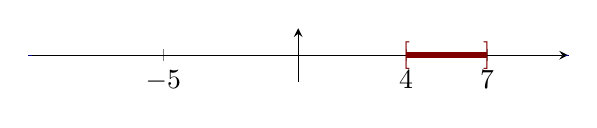
\begin{tikzpicture}
	\begin{axis}[
            %xmin=-25,xmax=25,ymin=-25,ymax=25,
            %width=3in,
            clip=false,
            axis lines=center,
            %ticks=none,
            unit vector ratio*=1 1 1,
            ymajorticks=false,
            xtick={-5,4, 7},
            %xlabel=$x$, ylabel=$y$,
            %every axis y label/.style={at=(current axis.above origin),anchor=south},
            every axis x label/.style={at=(current axis.right of origin),anchor=west},
          ]      
       
          	\addplot [line width=2, penColor2, smooth,samples=100,domain=(4:7)] ({x},{0});

          	\addplot [line width=0.5, penColor, smooth,samples=100,domain=(-10:-9.9)] ({x},{0});
          	\addplot [line width=0.5, penColor, smooth,samples=100,domain=(9.9:10)] ({x},{0});


          	\node at (axis cs:4,0) [penColor2] {$[$};
          	\node at (axis cs:7,0) [penColor2] {$]$};

    \end{axis}
	\end{tikzpicture}
	\end{image}





	\item All of the real numbers between $4$ and $7$, including $4$ but not $7$.  We use parenthese to indicate exclusion:  $[4, 7)$
	\begin{image}
	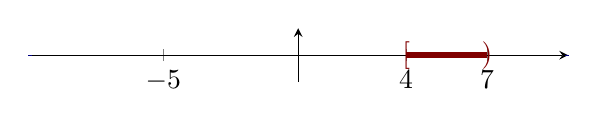
\begin{tikzpicture}
	\begin{axis}[
            %xmin=-25,xmax=25,ymin=-25,ymax=25,
            %width=3in,
            clip=false,
            axis lines=center,
            %ticks=none,
            unit vector ratio*=1 1 1,
            ymajorticks=false,
            xtick={-5,4, 7},
            %xlabel=$x$, ylabel=$y$,
            %every axis y label/.style={at=(current axis.above origin),anchor=south},
            every axis x label/.style={at=(current axis.right of origin),anchor=west},
          ]      
       
          	\addplot [line width=2, penColor2, smooth,samples=100,domain=(4:7)] ({x},{0});

          	\addplot [line width=0.5, penColor, smooth,samples=100,domain=(-10:-9.9)] ({x},{0});
          	\addplot [line width=0.5, penColor, smooth,samples=100,domain=(9.9:10)] ({x},{0});


          	\node at (axis cs:4,0) [penColor2] {$[$};
          	\node at (axis cs:7,0) [penColor2] {$)$};

    \end{axis}
	\end{tikzpicture}
	\end{image}




	\item All of the real numbers between $4$ and $7$, including $7$ but not $4$:   $(4, 7]$
	\begin{image}
	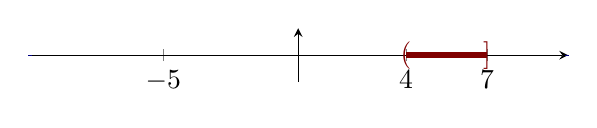
\begin{tikzpicture}
	\begin{axis}[
            %xmin=-25,xmax=25,ymin=-25,ymax=25,
            %width=3in,
            clip=false,
            axis lines=center,
            %ticks=none,
            unit vector ratio*=1 1 1,
            ymajorticks=false,
            xtick={-5,4, 7},
            %xlabel=$x$, ylabel=$y$,
            %every axis y label/.style={at=(current axis.above origin),anchor=south},
            every axis x label/.style={at=(current axis.right of origin),anchor=west},
          ]      
       
          	\addplot [line width=2, penColor2, smooth,samples=100,domain=(4:7)] ({x},{0});

          	\addplot [line width=0.5, penColor, smooth,samples=100,domain=(-10:-9.9)] ({x},{0});
          	\addplot [line width=0.5, penColor, smooth,samples=100,domain=(9.9:10)] ({x},{0});


          	\node at (axis cs:4,0) [penColor2] {$($};
          	\node at (axis cs:7,0) [penColor2] {$]$};

    \end{axis}
	\end{tikzpicture}
	\end{image}




	\item All of the real numbers between $4$ and $7$, including neither $4$ nor $7$:    $(4, 7)$
	\begin{image}
	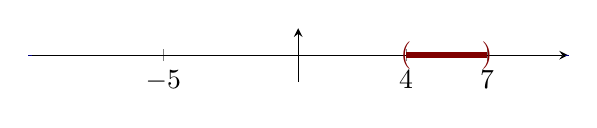
\begin{tikzpicture}
	\begin{axis}[
            %xmin=-25,xmax=25,ymin=-25,ymax=25,
            %width=3in,
            clip=false,
            axis lines=center,
            %ticks=none,
            unit vector ratio*=1 1 1,
            ymajorticks=false,
            xtick={-5,4, 7},
            %xlabel=$x$, ylabel=$y$,
            %every axis y label/.style={at=(current axis.above origin),anchor=south},
            every axis x label/.style={at=(current axis.right of origin),anchor=west},
          ]      
       
          	\addplot [line width=2, penColor2, smooth,samples=100,domain=(4:7)] ({x},{0});

          	\addplot [line width=0.5, penColor, smooth,samples=100,domain=(-10:-9.9)] ({x},{0});
          	\addplot [line width=0.5, penColor, smooth,samples=100,domain=(9.9:10)] ({x},{0});


          	\node at (axis cs:4,0) [penColor2] {$($};
          	\node at (axis cs:7,0) [penColor2] {$)$};

    \end{axis}
	\end{tikzpicture}
	\end{image}

	\end{itemize}



\begin{explanation} \textbf{Video: Interval Notation for Bounded Intervals}

[ Click on the arrow to the right to expand for the video. ]
\begin{expandable} 

\begin{center}
\youtube{orhSSkxM6bQ}
\end{center}

\end{expandable}
\end{explanation}




\item  \textbf{Building Block:} \textbf{\textcolor{purple!85!blue}{Infinite (Unbounded) Intervals}}  


Our subsets might include the right or left half of the real number line.  These are called \textbf{infinite intervals} or \textbf{unbounded intervals}.   Infinite intervals include \textbf{\textcolor{red!90!darkgray}{ALL}} of the real numbers less than a specific real number, or \textbf{\textcolor{red!90!darkgray}{ALL}} of the real numbers greater than a specific real number. 

	\begin{itemize}
	\item All of the real numbers less than $4$ and including $4$.  When writing, we use negative infinity, -$\infty$, to indicate the interval extends without end, $(-\infty, 4]$.  When drawing, we use a left arrow.
	\begin{image}
	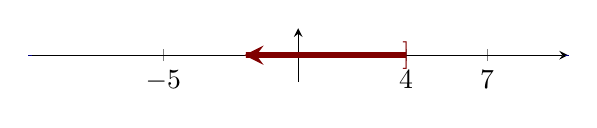
\begin{tikzpicture}
	\begin{axis}[
            %xmin=-25,xmax=25,ymin=-25,ymax=25,
            %width=3in,
            clip=false,
            axis lines=center,
            %ticks=none,
            unit vector ratio*=1 1 1,
            ymajorticks=false,
            xtick={-5,4, 7},
            %xlabel=$x$, ylabel=$y$,
            %every axis y label/.style={at=(current axis.above origin),anchor=south},
            every axis x label/.style={at=(current axis.right of origin),anchor=west},
          ]      
       
          	\addplot [line width=2, penColor2, smooth,samples=100,domain=(-2:4),<-] ({x},{0});

          	\addplot [line width=0.5, penColor, smooth,samples=100,domain=(-10:-9.9)] ({x},{0});
          	\addplot [line width=0.5, penColor, smooth,samples=100,domain=(9.9:10)] ({x},{0});


          	\node at (axis cs:4,0) [penColor2] {$]$};

    \end{axis}
	\end{tikzpicture}
	\end{image}


\item All of the real numbers less than $4$ but not including $4$, $(-\infty, 4)$
	\begin{image}
	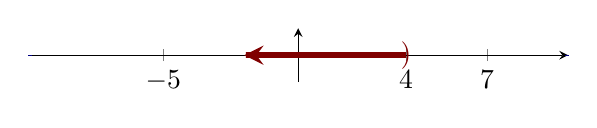
\begin{tikzpicture}
	\begin{axis}[
            %xmin=-25,xmax=25,ymin=-25,ymax=25,
            %width=3in,
            clip=false,
            axis lines=center,
            %ticks=none,
            unit vector ratio*=1 1 1,
            ymajorticks=false,
            xtick={-5,4, 7},
            %xlabel=$x$, ylabel=$y$,
            %every axis y label/.style={at=(current axis.above origin),anchor=south},
            every axis x label/.style={at=(current axis.right of origin),anchor=west},
          ]      
       
          	\addplot [line width=2, penColor2, smooth,samples=100,domain=(-2:4),<-] ({x},{0});

          	\addplot [line width=0.5, penColor, smooth,samples=100,domain=(-10:-9.9)] ({x},{0});
          	\addplot [line width=0.5, penColor, smooth,samples=100,domain=(9.9:10)] ({x},{0});


          	\node at (axis cs:4,0) [penColor2] {$)$};

    \end{axis}
	\end{tikzpicture}
	\end{image}


\item All of the real numbers greater than $4$ and including $4$.  When writing, we use positive infinity, $\infty$, to indicate the interval extends without end, $[4, \infty)$. When drawing, we use a right arrow.
	\begin{image}
	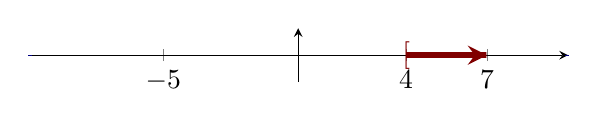
\begin{tikzpicture}
	\begin{axis}[
            %xmin=-25,xmax=25,ymin=-25,ymax=25,
            %width=3in,
            clip=false,
            axis lines=center,
            %ticks=none,
            unit vector ratio*=1 1 1,
            ymajorticks=false,
            xtick={-5,4, 7},
            %xlabel=$x$, ylabel=$y$,
            %every axis y label/.style={at=(current axis.above origin),anchor=south},
            every axis x label/.style={at=(current axis.right of origin),anchor=west},
          ]      
       
          	\addplot [line width=2, penColor2, smooth,samples=100,domain=(4:7),->] ({x},{0});

          	\addplot [line width=0.5, penColor, smooth,samples=100,domain=(-10:-9.9)] ({x},{0});
          	\addplot [line width=0.5, penColor, smooth,samples=100,domain=(9.9:10)] ({x},{0});


          	\node at (axis cs:4,0) [penColor2] {$[$};

    \end{axis}
	\end{tikzpicture}
	\end{image}


\item All of the real numbers greater than $4$ but not including $4$, $(4, \infty)$.
	\begin{image}
	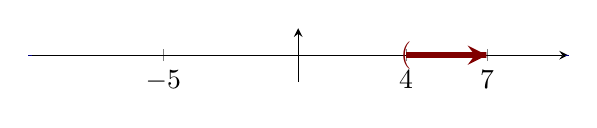
\begin{tikzpicture}
	\begin{axis}[
            %xmin=-25,xmax=25,ymin=-25,ymax=25,
            %width=3in,
            clip=false,
            axis lines=center,
            %ticks=none,
            unit vector ratio*=1 1 1,
            ymajorticks=false,
            xtick={-5,4, 7},
            %xlabel=$x$, ylabel=$y$,
            %every axis y label/.style={at=(current axis.above origin),anchor=south},
            every axis x label/.style={at=(current axis.right of origin),anchor=west},
          ]      
       
          	\addplot [line width=2, penColor2, smooth,samples=100,domain=(4:7),->] ({x},{0});

          	\addplot [line width=0.5, penColor, smooth,samples=100,domain=(-10:-9.9)] ({x},{0});
          	\addplot [line width=0.5, penColor, smooth,samples=100,domain=(9.9:10)] ({x},{0});


          	\node at (axis cs:4,0) [penColor2] {$($};

    \end{axis}
	\end{tikzpicture}
	\end{image}

	\end{itemize}

\end{itemize}



\textbf{Note:} $-\infty$ and $\infty$ are not real numbers, therefore they are never included in any set of real numbers.  $-\infty$ and $\infty$ are used as communication symbols. They let us know the intervals are \textbf{unbounded}. Therefore, they always have parentheses.  Square brackets are never used for $-\infty$ or $\infty$.



\begin{explanation} \textbf{Video: Interval Notation for Unbounded Intervals}

[ Click on the arrow to the right to expand for the video. ]
\begin{expandable} 

\begin{center}
\youtube{mLUjZgv8nO4}
\end{center}

\end{expandable}
\end{explanation}










\begin{definition} \item \textbf{\textcolor{green!50!black}{Bounded and Unbounded}}

Let $S$ be a subset of the real numbers. \\


\begin{itemize}
\item The set $S$ is \textbf{bounded from above}, if there exists a real number, $B$, such that for all $s \in S$, we have $s \leq B$.  There is a real number greater than or equal to all of the numbers in $S$.  \\

\item The set $S$ is \textbf{unbounded from above}, if for any selected real number, $B$, there exists $s \in S$, such that $B < s$. No matter how high the bar is set, $S$ contains a number greater than the bar.  \\

\item The set $S$ is \textbf{bounded from below}, if there exists a real number, $B$, such that for all $s \in S$, we have $B \leq s$.  There is a real number less than or equal to all of the numbers in $S$.  \\

\item The set $S$ is \textbf{unbounded from below}, if for any selected real number, $B$, there exists $s \in S$, such that $s < B$. No matter how low the bar is set, $S$ contains a number less than the bar.  \\

\item The set $S$ is \textbf{bounded}, if it is both bounded from above and below.  

\item The set $S$ is \textbf{unbounded}, if it is not bounded.  \\
\end{itemize}


\end{definition}






\subsection*{Interval Notation}

In the examples above, we used \textbf{interval notation} to describe the intervals in writing. Interval notation adheres to a few rules.

\begin{itemize}
\item For finite intervals, write the two extreme interval numbers in the order they would appear on the number line, separated by a comma.  These are called \textbf{endpoints} of the intervals.
\item Use a square bracket to indicate an endpoint is included in the interval.
\item Use a parenthesis to indicate an endpoint is excluded from the interval.
\item For infinite (unbounded) intervals, use $-\infty$ to indicate the interval extends without end to the left. $-\infty$ always appears on the left side. $-\infty$ always has a parenthesis around it, because $-\infty$ is not a real number and thus cannot be included in an interval of real numbers.
\item For infinite (unbounded) intervals use $\infty$ to indicate the interval extends without end to the right. $\infty$ always appears on the right side. $\infty$ always has a parenthesis around it, because $\infty$ is not a real number and thus cannot be included in an interval of real numbers. 
\end{itemize}


\begin{question}
Which is valid interval notation?
	\begin{multipleChoice}
	\choice {$[3, -2)$}
	\choice [correct]{$[-2, 3)$}
	\end{multipleChoice}
\end{question}



\begin{question}
Which is valid interval notation?
	\begin{multipleChoice}
	\choice {$[1, \infty]$}
	\choice [correct]{$[1, \infty)$}
	\end{multipleChoice}
\end{question}



\begin{question}
Select all that have valid interval notation.
	\begin{selectAll}
	\choice {$[-3, -5]$}
	\choice [correct]{$[1, 8)$}
	\choice [correct]{$(-\infty, -4]$}
	\choice {$[-\infty, 7)$}
	\choice [correct]{$(-3, 3)$}
	\choice [correct]{$(-1, 2]$}
	\choice {$[6, 2]$}
	\end{selectAll}
\end{question}


\begin{warning}  \textbf{\textcolor{red!80!black}{Numbers vs. Points}} \\

Many people in many countries over many centuries have studied mathematics and invented language to communicate their findings. This is a problem for us. We are stuck with their language, even though it might not be what we would have selected. They had their reasons.  We live with their reasons.\\

On our number line we plot dots to represent numbers and we call these points.  They are points on the number line, because a point identifies a location.  We will soon represent our functions with 2-dimensional drawings. We will still have points and they will still identify a location.  However, with two dimensions, describing the location will require two numbers, rather than one.  A point will no longer represent a single number.\\

Our language will become a little blurred when we talk about points versus numbers.  Just be aware that our language is old and has been twisted to accommodate many thoughts by many people.\\


We will attempt to keep the blur to a miminum in this course by our judicial use of the words \textit{number} and \textit{point}.

\textbf{Note:} We will reserve the word ``point'' for graphical descriptions and ``number'' for algebraic communication.
\end{warning}








\begin{notation}  \textbf{\textcolor{blue!55!black}{membership}} 

Now that we can describe sets of numbers with interval notation, we can use our membership symbol, $\in$, to communicate when individual numbers are included in the interval or when they are not included, $\notin$.

\end{notation}








\begin{question}
Which is a valid statement?
    \begin{multipleChoice}
    \choice {$ 2 \in [3, -2)$}
    \choice [correct]{$-2 \in [-2, 3)$}
    \end{multipleChoice}
\end{question}



\begin{question}
Which is a valid statement?
    \begin{multipleChoice}
    \choice {$3 \notin [1, \infty]$}
    \choice [correct]{$-3 \notin [1, \infty)$}
    \end{multipleChoice}
\end{question}



\begin{question}
Select all valid statements.
    \begin{selectAll}
    \choice {$4 \in [-3, -5]$}
    \choice [correct]{$4 \in [1, 8)$}
    \choice [correct]{$5 \notin (-\infty, -4]$}
    \choice {$0 \notin [-\infty, 7)$}
    \choice [correct]{$0 \in (-3, 3)$}
    \choice [correct]{$0 \in (-1, 2]$}
    \choice {$0 \in [6, 2]$}
    \end{selectAll}
\end{question}








\begin{definition} \textbf{\textcolor{green!50!black}{Open Intervals}}

Intervals of the form $(a, b)$, $(-\infty, b)$, or $(a, \infty)$ are called \textbf{open intervals}.

\end{definition}



\begin{definition} \textbf{\textcolor{green!50!black}{Closed Intervals}}

Intervals of the form $[a, b]$, $(-\infty, b]$, or $[a, \infty)$ are called \textbf{closed intervals}.

\end{definition}




\begin{warning}

$(-\infty, \infty)$ is both an open interval and a closed interval.


\end{warning}




\begin{definition} \textbf{\textcolor{green!50!black}{The Empty Set}}

\textbf{The empty set} is the set containing no numbers.  $\emptyset$ and $\{  \, \}$ are both symbols for the empty set.

\end{definition}







\subsection*{Set Builder Notation}

A second way to represent intervals in writing is with inequalities. However, we cannot simply insert an inequality into our description, because people use inequalities in several contexts.  So, we need some notation that tells people we are describing a set. \textbf{Set builder notation} includes shorthand symbols to represent sentences such as 

\begin{center}
``The set of all real numbers such that the numbers are greater than or equal to 4 and less than 7.''
\end{center}

We begin with a pair of curly braces $\{  \, \}$ containing a vertical bar:  ${|}$.  The vertical bar separates two areas inside the curly braces. The left area is where we describe the types of numbers we are working with (real, integers, rational, etc).  The right area is where we place our inequality.





\begin{explanation} \textbf{Video: Interval Notation, Inequalities, and Graphs}

[ Click on the arrow to the right to expand for the video. ]
\begin{expandable} 

\begin{center}
\youtube{dZzid5L5pvk}
\end{center}

\end{expandable}
\end{explanation}





\begin{example}
``The set of all real numbers such that the numbers are greater than or equal to 4 and less than 7.''
\[ \{ r \in \mathbb {R} \, | \, (4 \leq r)  \text{ and } (r < 7) \} \]
\[ \{ r \in \mathbb {R} \, | \, 4 \leq r < 7 \} \]

\begin{warning}
\textbf{ALL} real numbers would include numbers such as $5$, $\frac{17}{4}$, $\sqrt{19}$, $6.354987263$, and $211^{\tfrac{1}{\pi}}$, not just whole numbers.
\end{warning}
\end{example}



\begin{example}
``The set of all integers such that the numbers are greater than or equal to 4 and less than 7.''
\[ \{ n \in \mathbb {Z} \, | \, 4 \leq n < 7 \} \]

\begin{explanation}
This would be the set $\{ 4, 5, 6 \}$.
\end{explanation}
\end{example}




\begin{question}
Select the interval notation that describes the same set as 
\[ \{ t \in \mathbb {R} \, | \, 2 < t \leq 9 \} \]
	\begin{multipleChoice}
	\choice {$[9, 2)$}
	\choice {$[2, 9)$}
	\choice [correct]{$(2, 9]$}
	\choice {$[2, 9]$}
	\choice {$(2, 9)$}
	\end{multipleChoice}
\end{question}





\begin{question}
Complete the interval notation that describes the same set as 
\[ \{ r \in \mathbb {R} \, | \, -3 \leq r < 7 \} \]

\[
\left [ \answer{-3} , \answer{7} \right )
\]



\end{question}




















\subsection*{Gluing Building Blocks Together: Unions}

Our building blocks for sets of real numbers are lists of individual numbers along with intervals.  We can combine these to describe any set of real numbers that we need.  These combinations are called \textbf{unions}.  The union symbol is $\cup$. Unions are usually written with interval notation.



\begin{definition} \textbf{\textcolor{green!50!black}{Union}}

The \textbf{union} of two sets is a set containing all elements from both sets.


\[
A \cup B = \{  x \, | \, (x \in A) \, \text{ or } \, (x \in B)  \}
\]


\end{definition}





\begin{definition} \textbf{\textcolor{green!50!black}{Intersection}}

The \textbf{intersecton} of two sets is a set containing all elements common in both sets.


\[
A \cap B = \{  x \, | \, (x \in A) \, \text{ and } \, (x \in B)  \}
\]


\end{definition}




\begin{explanation} \textbf{Video: Sets}

[ Click on the arrow to the right to expand for the video. ]
\begin{expandable} 

\begin{center}
\youtube{Z1ebRZ36jJI}
\end{center}

\end{expandable}
\end{explanation}



\begin{explanation} \textbf{Video: Singletons}

[ Click on the arrow to the right to expand for the video. ]
\begin{expandable} 

\begin{center}
\youtube{LySOpHA7iwk}
\end{center}

\end{expandable}
\end{explanation}




\begin{example}

\[ [-4, -2] \cup \{ 2 \} \cup (3, 6] \]

\begin{image}
	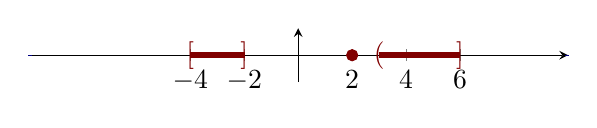
\begin{tikzpicture}
	\begin{axis}[
            %xmin=-25,xmax=25,ymin=-25,ymax=25,
            %width=3in,
            clip=false,
            axis lines=center,
            %ticks=none,
            unit vector ratio*=1 1 1,
            ymajorticks=false,
            xtick={-4,-2,2,4, 6},
            %xlabel=$x$, ylabel=$y$,
            %every axis y label/.style={at=(current axis.above origin),anchor=south},
            every axis x label/.style={at=(current axis.right of origin),anchor=west},
          ]      
       
          	\addplot [line width=2, penColor2, smooth,samples=100,domain=(-4:-2)] ({x},{0});
			\addplot [line width=2, penColor2, smooth,samples=100,domain=(3:6)] ({x},{0});
          	\addplot [color=penColor2,only marks,mark=*] coordinates{(2,0)};

          	\addplot [line width=0.5, penColor, smooth,samples=100,domain=(-10:-9.9)] ({x},{0});
          	\addplot [line width=0.5, penColor, smooth,samples=100,domain=(9.9:10)] ({x},{0});


          	\node at (axis cs:-4,0) [penColor2] {$[$};
          	\node at (axis cs:-2,0) [penColor2] {$]$};
          	\node at (axis cs:3,0) [penColor2] {$($};
          	\node at (axis cs:6,0) [penColor2] {$]$};

    \end{axis}
	\end{tikzpicture}
	\end{image}

\end{example}




\begin{example}

\[ (-\infty, -1]  \cup (4, 8) \]

\begin{image}
	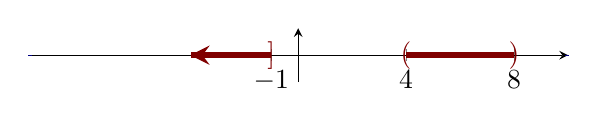
\begin{tikzpicture}
	\begin{axis}[
            %xmin=-25,xmax=25,ymin=-25,ymax=25,
            %width=3in,
            clip=false,
            axis lines=center,
            %ticks=none,
            unit vector ratio*=1 1 1,
            ymajorticks=false,
            xtick={-1, 4, 8},
            %xlabel=$x$, ylabel=$y$,
            %every axis y label/.style={at=(current axis.above origin),anchor=south},
            every axis x label/.style={at=(current axis.right of origin),anchor=west},
          ]      
       
          	\addplot [line width=2, penColor2, smooth,samples=100,domain=(-4:-1),<-] ({x},{0});
			\addplot [line width=2, penColor2, smooth,samples=100,domain=(4:8)] ({x},{0});
          	%\addplot [color=penColor2,only marks,mark=*] coordinates{(2,0)};

          	\addplot [line width=0.5, penColor, smooth,samples=100,domain=(-10:-9.9)] ({x},{0});
          	\addplot [line width=0.5, penColor, smooth,samples=100,domain=(9.9:10)] ({x},{0});


          	\node at (axis cs:-1,0) [penColor2] {$]$};
          	\node at (axis cs:4,0) [penColor2] {$($};
          	\node at (axis cs:8,0) [penColor2] {$)$};

    \end{axis}
	\end{tikzpicture}
	\end{image}

\end{example}




\begin{example}

\[ (-7, -4] \cup \{ -1, 1 \} \cup (3, \infty) \]

	\begin{image}
	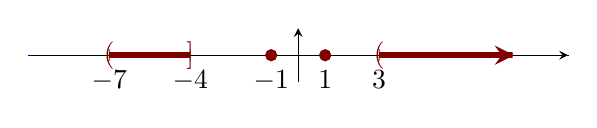
\begin{tikzpicture}
	\begin{axis}[
            %xmin=-25,xmax=25,ymin=-25,ymax=25,
            %width=3in,
            clip=false,
            axis lines=center,
            %ticks=none,
            unit vector ratio*=1 1 1,
            ymajorticks=false,
            xtick={-7,-4,-1,1,3},
            %xlabel=$x$, ylabel=$y$,
            %every axis y label/.style={at=(current axis.above origin),anchor=south},
            every axis x label/.style={at=(current axis.right of origin),anchor=west},
          ]      
       
          	\addplot [line width=2, penColor2, smooth,samples=100,domain=(3:8),->] ({x},{0});
			\addplot [line width=2, penColor2, smooth,samples=100,domain=(-7:-4)] ({x},{0});
          	\addplot [color=penColor2,only marks,mark=*] coordinates{(-1,0)};
          	\addplot [color=penColor2,only marks,mark=*] coordinates{(1,0)};

          	\addplot [line width=0.5, penColor, smooth,samples=100,domain=(-10:-9.9)] ({x},{0});
          	\addplot [line width=0.5, penColor, smooth,samples=100,domain=(9.9:10)] ({x},{0});


          	\node at (axis cs:-7,0) [penColor2] {$($};
          	\node at (axis cs:-4,0) [penColor2] {$]$};
          	\node at (axis cs:3,0) [penColor2] {$($};

    \end{axis}
	\end{tikzpicture}
	\end{image}

\end{example}





\begin{question}
Select the interval notation that describes the same set as the following graph.
	\begin{image}
	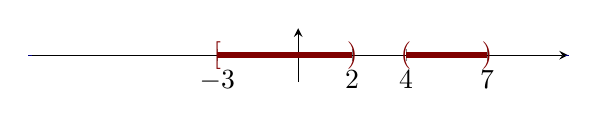
\begin{tikzpicture}
	\begin{axis}[
            %xmin=-25,xmax=25,ymin=-25,ymax=25,
            %width=3in,
            clip=false,
            axis lines=center,
            %ticks=none,
            unit vector ratio*=1 1 1,
            ymajorticks=false,
            xtick={-3,2,4,7},
            %xlabel=$x$, ylabel=$y$,
            %every axis y label/.style={at=(current axis.above origin),anchor=south},
            every axis x label/.style={at=(current axis.right of origin),anchor=west},
          ]      
       
          	\addplot [line width=2, penColor2, smooth,samples=100,domain=(-3:2)] ({x},{0});
			\addplot [line width=2, penColor2, smooth,samples=100,domain=(4:7)] ({x},{0});

          	\addplot [line width=0.5, penColor, smooth,samples=100,domain=(-10:-9.9)] ({x},{0});
          	\addplot [line width=0.5, penColor, smooth,samples=100,domain=(9.9:10)] ({x},{0});


          	\node at (axis cs:-3,0) [penColor2] {$[$};
          	\node at (axis cs:2,0) [penColor2] {$)$};
          	\node at (axis cs:4,0) [penColor2] {$($};
          	\node at (axis cs:7,0) [penColor2] {$)$};

    \end{axis}
	\end{tikzpicture}
	\end{image}


	\begin{multipleChoice}
	\choice {$(-3, 2) \cup (4, 7)$}
	\choice {$[-3, 2) (4, 7)$}
	\choice {$(-3, 2] \cup [4, 7]$}
	\choice [correct]{$[-3, 2) \cup (4, 7)$}
	\choice {$[-3, 2), (4, 7)$}
	\end{multipleChoice}
\end{question}





















\subsection*{Reduced Form}

All of the following describe the same set.

\begin{itemize}
\item $[-2, 2)$
\item $[-2, -1] \cup (-1, 2)$
\item $[-2, -1) \cup [-2, 0) \cup [-2, 1) \cup [-2, 2)$
\item $[-2, 0) \cup \{ 0 \} \cup (0, 2)$
\item $[-2, 0) \cup \{ 0 \} \cup (0, 1) \cup \{ 1 \} \cup (1, 2)$
\item $[-2, 0) \cup [-1, 1) \cup [1, 2)$
\end{itemize}

Having such a wide variety of descriptions is very valuable as we move through mathematics.  However, for communication purposes, it causes confusion. Therefore, we are establishing an official reduced form for interval notation.  We will always use the reduced form, unless there is a good reason not to.  (There are often good reasons.)

Our reduced form will adhere to some rules:





\begin{notation} \textbf{\textcolor{blue!75!black}{Reduced Interval Notation}} \\

\begin{itemize}
\item Do not use overlapping or intersecting intervals.
\item Do not list individual numbers that are members of an interval.
\item Do not list individual numbers that can be used as endpoints of an interval.
\item Write the intervals and sets of individual numbers in proper numeric order.
\end{itemize}

\end{notation}
Communication!

Our reduced form of interval notation mimics exactly what you would draw on a number line.







\begin{explanation} \textbf{Video: Reduced Interval Notation}

[ Click on the arrow to the right to expand for the video. ]
\begin{expandable} 

\begin{center}
\youtube{5mLnsbfmLtI}
\end{center}

\end{expandable}
\end{explanation}




\begin{question}
Select all of the unions that are written in reduced form.
  \begin{selectAll}
  \choice [correct]{$(-3, 2) \cup (4, 7)$}
  \choice {$[-3, 4) \cup (2, 7)$}
  \choice {$(-3, 2] \cup [4, 7] \cup \{ 3 \}$}
  \choice [correct]{$[-3, 2) \cup \{ 3 \} \cup (4, 7)$}
  \choice {$(4, 7) \cup [-3, 2)$}
  \end{selectAll}
\end{question}




\begin{definition} \textbf{\textcolor{green!50!black}{Maximal Intervals}}

When a set of real numbers is written in reduced form, then each of the intervals is called a \textbf{maximal interval} of the set.
\end{definition}
Maximal intervals cannot be made larger inside the set.  


\begin{example} Maximal Intervals \\
Let $S = [-3, 2) \cup \{ 3 \} \cup (4, 7)$, then

\begin{itemize}
\item $[-3, 2)$ is a maximal interval of $S$.
\item $(4, 7)$ is a maximal interval of $S$.
\end{itemize}


$3$ is an isolated number of $S$, \\

$-3$, $2$, $4$, and $7$ are all endpoints of maximal intervals of $S$. \\

$-3$ is the only included endpoint of a maximal interval of $S$.



\end{example}
Endpoints are usually the focus of maximal intervals.







\begin{example} nonMaximal Intervals \\
Let $S = [-4, 1) \cup \{ 1, 4 \} \cup (5, 9)$, then


$(-3, 1)$ is not a maximal interval of $S$.

We can extend this interval to $[-3, 1)$ and still stay inside $S$.


\end{example}
Of course, we could have also extended $(-3, 1)$ to the maximal interval it sits inside, $(-3, 1) \subset [-4, 1)$. \\

Maximal intervals give us information about the structure of the domain of functions.

















\begin{center}
\textbf{\textcolor{green!50!black}{ooooo-=-=-=-ooOoo-=-=-=-ooooo}} \\

more examples can be found by following this link\\ \link[More Examples of Real-Valued Functions]{https://ximera.osu.edu/csccmathematics/precalculus1/precalculus1/realValued/examples/exampleList}

\end{center}








\end{document}
